\section{Openlayers}
\label{sec:Openlayer}

Openlayers ist eine leistungfähige Open Source JavaScript Bibliothek und ein vielseitiges Werkzeug zur Visualisierung von Karten in der webbasierten Anwendungen. Raster- und Vektordaten von verschiedenen Kartenanbieter könnten mit Hilfe von dieser Bibliothek dynamische und interaktive Karten in Webseiten eingebunden und angepasst werden. Als Open Source Projekt wird OpenLayers ständig von einer aktiven Community weiterentwickelt und verbessert. Dies gewährleistet regelmäßige Updates und eine breite Palette von Funktionen.\\

Werkzeugkasten von OpenLayers erfühlt sehr viele unterschiedlichen Aufgaben. Die wichtigsten Kernfuntionen sind:
\begin{itemize}
    \item Unterstützung verschiedener Kartenquellen:
    \begin{itemize}
        \item Raster: WMS/WMTS, OpenStreetMap, MapQuest, Stamen, Bing, statische Bilder usw.
        \item Vektor: WFS, KmL, GeoJSON, TopoJSON, MapBox Vector Tiles usw.
    \end{itemize}
    \item Layer-Management: umfassende Möglichkeiten zum Verwalten verschiedener Kartenebenen (Layers). Es könnten mehrere Ebenen wie Satellitenbilder, Straßenkarten, Wetterdaten oder geographische Daten überlagert und gesteuert werden.
    \item Bedienelemente (Controls) und Interaktionen (Draws): Übersichtskarten, Schieberegler zu Zoomen, Drehen, Objektauswahl, Zeichnen auf der Karte
    \item Overlays: Darstellungen der DOM Elemente an jeder Position der Karte sowie Erzeugung von Tooltips und Marker.
    \item Stilisierung und Rendering: Es möglicht individuelles Styling von Karten und Geojbjekten zu definieren, anzupassen und untershiedliche Daten und Information hervorzuheben.
    \item Geographische Funktionen: Berechnungen wie Distanzmessung, Flächenberechnung und Transformation zwischen verschiedenen Koordinatensystemen sowie Umprojektionierungen.
    \item Ereignisse: Anbringen von Listener Funktionen zur Reaktion auf Ereignisse auf der Karte.
    \item Erweiterbarkeit, Anpassungsfähigkeit und mobile Unterstüztung.
\end{itemize}

In der Abbildung 2.6 werden beispielsweise einige der genannten Funktionen illustriert. In diesem Screenshot sind unterschiedlichen Ebenen zu sehen: OpenStreetMap, zwei thematische Geodaten (jeweil als ein Layer dargestellt) und die Bedienelemente, mit deren Hilfe jeder Layer gesteuert werden könnte.

\begin{figure}[ht]
  \centering
  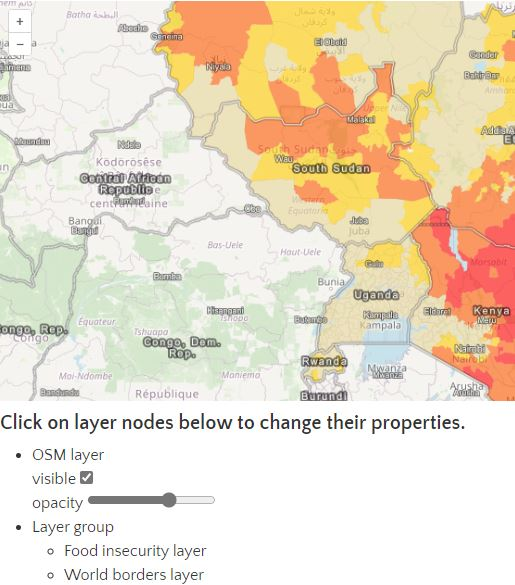
\includegraphics[width=\linewidth]{images/layer-group.JPG}
  \caption{OpenLayers - Layer Group \citep{openlayers_examples}}
  \label{fig:meineabbildung}
\end{figure}
Im Kapitel 5 werden die oben genannten Funktionen näher beschrieben und erklärt. In der praktischen Umsetzung des Showcases, bei dem ein GIS für ein Formular erstellt wird, kamen all diese Funktionen von OpenLayers zum Einsatz. 



